\documentclass[10pt,a4paper]{article}
\usepackage[utf8]{inputenc}
\usepackage[spanish]{babel}
\usepackage{amsmath}
\usepackage{amsfonts}
\usepackage{amssymb}
\usepackage{graphicx}
\usepackage[left=2cm,right=2cm,top=2cm,bottom=2cm]{geometry}
\usepackage[hidelinks]{hyperref}
\usepackage{listings}

\lstset { frame = single, breaklines = true }


\begin{document}

\begin{titlepage}
\title{\textbf{
	{\Huge Práctica 4: Vulnerabilidades de desbordamiento}\\
	{\Large Seguridad Informática}
}}
\author{
	Pedro Allué Tamargo (758267)
	\and
	Juan José Tambo Tambo (755742)
}
\date{\today}
\clearpage\maketitle
\thispagestyle{empty}
\tableofcontents
\end{titlepage}

\section{Identificación de vulnerabilidades}

\subsection{Hay una vulnerabilidad asociada a una variable que puede ser indexada fuera de su límite}
\begin{itemize}
\item ¿Cuál es la variable?
	\begin{itemize}
	\item La variable es \texttt{func}. Esta variable almacena un \emph{array} de punteros a funciones que devuelven \texttt{void} y no aceptan parámetros.
	\item Ejecutando el programa sin las contramedidas, cuando pide la introducción de una opción del menú, se introduce la opción 6 y se indexa el \emph{array} \texttt{funcsec}, declarado en direcciones contiguas.
	\end{itemize}
\item Indicar la línea de código que puede indexar la variable fuera de su límite.
	\begin{itemize}
	\item La variable se puede indexar fuera de su límite en la línea 131.
	\end{itemize}
\end{itemize}


\subsection{Hay vulnerabilidades de desbordamiento de búfer en el programa}
\begin{itemize}
\item ¿Cuáles son las variables?
	\begin{itemize}
	%\item La variable \texttt{resp} en la función \texttt{main}. Acepta cadenas de caracteres de hasta 512 \emph{bytes} de longitud. \textbf{(?)}
	\item La variable \texttt{comida} en la función \texttt{llenarCarrito}. Acepta 512 \emph{bytes} de longitud pero la función \texttt{scanf} no establece un límite para controlar la longitud de la cadena a copiar.
	\item La variable \texttt{malo} en la función \texttt{mostrarCalorias} utiliza una versión no segura de la función \texttt{strlen} que devuelve el número de bytes (caracteres) entre una dirección de inicio y el carácter terminador \texttt{0}. Si esta longitud es mayor que 512 (\emph{MAX\_{}SIZE}) se copiarán tantos caracteres como diga \texttt{len} o hasta llegar al carácter terminador.
	\end{itemize}
\item ¿Qué parte de la memoria asociada al proceso se puede desbordar?
	\begin{itemize}
	\item Se podría desbordar la pila. Al ser variables que se declaran en funciones y no son globales se almacenan en la pila.
	\end{itemize}
\item Indicar las líneas de código que pueden desbordar los búferes.
	\begin{itemize}
%	\item \texttt{resp}: el acceso a los datos de otro \emph{array} (\texttt{funcsec}) en la línea \textbf{nLinea}.
	\item \texttt{comida}: la función \texttt{scanf} (línea 58)
	\item \texttt{malo}: la función \texttt{strlen} (línea 86) junto con la función \texttt{strncat}  (línea 87).
	\end{itemize}
\end{itemize}


\subsection{¿Hay otros tipos de vulnerabilidades en el código? ¿Cuáles?}
\begin{itemize}
\item Hay una vulnerabilidad de desbordamiento de enteros en la función \texttt{mostrarCalorías}, en la línea 90 (variable \texttt{total}). Dada una lista de comidas lo suficientemente grande, y debido al bucle \texttt{for} de la línea 81 se podría desbordar el valor de esta variable.
\item Existe otra vulnerabilidad de desbordamiento de enteros relacionada con la elección de la opción del menú del usuario (línea 127) puede desbordar el valor del entero \texttt{s} (función \texttt{atoi}, línea 130) si \texttt{resp} no se puede representar en el rango de los enteros (\texttt{int}). Una solución sería utilizar la función \texttt{strtol} que convierte una cadena de texto a un entero tipo \texttt{long} y ante desbordamientos, devuelve los límites máximos o mínimos del tipo \texttt{long}, dependiendo de por donde ha desbordado.
\end{itemize}


\section{Redirección de la ejecución}

\subsection{¿Cuál es la dirección de las variables \texttt{func} y \texttt{funcsec}? ¿En qué parte de la memoria se encuentran?}

Para obtener la localización de las variables en memoria mediante \texttt{gdb} se utilizará la orden: \texttt{print \&{}variable}. Por lo tanto, las direcciones de las variables serán las siguientes:
\begin{itemize}
\item La variable \texttt{func} se encuentra en la dirección \emph{0x804b064}
\item La variable \texttt{funcsec} se encuentra en la dirección \emph{0x804b078}
\end{itemize}

Las variables se encuentran en la zona de datos inicializados (\emph{Initialized Data Segment}) ya que son variables globales cuyo valor ha sido otorgado por el programador.


\subsection{¿Cuál es la dirección del método \texttt{showSecret1}?}

Para obtener la dirección de la función \texttt{showSecret1} mediante \texttt{gdb} se ha utilizado la siguiente orden: \texttt{print \&{}Carrito::mostrarSecreto1}. Ya que \texttt{mostrarSecreto1} es un método estático de la clase \texttt{Carrito}. Su dirección de memoria es: \emph{0x8048bce}.


\subsection{¿Qué datos de entrada proporcionas al programa para que \texttt{func[s]} lea el puntero a la función guardado en \texttt{funcsec}, en lugar de un puntero a una función guardado en \texttt{func}?}

La entrada proporcionada al programa para leer un puntero guardado en \texttt{funcsec} sería de al menos 5. Esto es así ya que la dirección inicial de \texttt{func} es \emph{0x804b064} y almacena punteros, cuyo tamaño son 4 \emph{bytes}. Para leer un puntero de \texttt{funcsec} habría que indexar la quinta posición (empezando por 0) de \texttt{func} (\emph{0x804b064 + (5*size\_{}puntero) = 0x804b078}).\\

\begin{figure}[h!]`
\centering
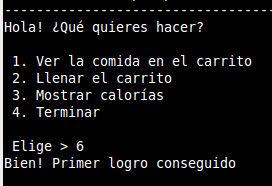
\includegraphics[scale=0.8]{images/primer_logro.png}
\caption{Captura de pantalla del resultado de la ejecución de \texttt{mostraSecreto1}}
\label{fig:mostrarSecreto1}
\end{figure}


\section{Ejecución del método \texttt{mostrarSecreto2}}

\subsection{¿Cuál es la dirección del búfer asociado a la variable \texttt{resp}?}

Para conseguir la dirección de memoria de la variable \texttt{resp} mediante \texttt{gdb} se utilizarán los siguientes comandos. El comando \texttt{backtrace} (\texttt{bt}) servirá para obtener la pila de ejecución (\emph{backtrace}) del programa (Figura \textbf{numFigura}). Tras esto se ejecutará el comando \texttt{frame 9} (\texttt{f 9}). Este comando establecerá el contexto al de la función \texttt{main}. Una vez situados en este contexto se ejecutará \texttt{print \&{}main::resp}. La dirección de memoria asociada a la variable \texttt{resp} será: \emph{0xbffff34f}\\

\begin{figure}[h!]
\centering
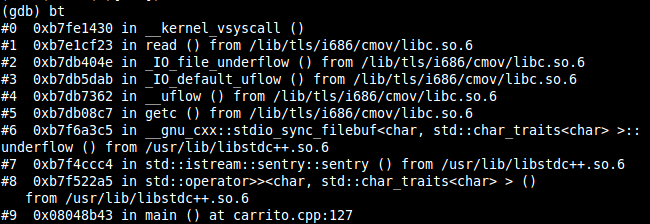
\includegraphics[scale=0.8]{images/bt.png}
\caption{Captura de pantalla de la salida de la orden \emph{backtrace} (\emph{bt})}
\label{fig:bt}
\end{figure}


\subsection{¿Qué datos de entrada proporcionas al programa para que \texttt{func[s]} lea a partir del 126º byte en \texttt{resp}, es decir, a partir de \texttt{resp[125]}?}

Dirección de \texttt{mostrarSecreto2} = \emph{0x08048a54}\\
Dirección de \texttt{resp} = \emph{0xbffff34f}\\
Dirección de \texttt{func} = \emph{0x0804b064}\\

YYYYYY = 771674330\\
Tiene que haber x A's\\
XE = Dir. mostrarSecreto2\\

Por lo tanto, me cagon dioooooooooos \textbf{completar}\\



\subsection{¿Hay otra forma de conseguir la escritura del segundo mensaje secreto por pantalla?}

Dirección de \texttt{mostrarSecreto2} = \emph{0x08048a54}\\
Dirección \texttt{saved eip} = \emph{0xb7d5f775}\\
Dirección de \texttt{eip} = \emph{0xbffff558}\\
Entre \emph{resp} y \emph{saved eip} hay 525 \emph{bytes}\\
Hay que hacer que resp desborde la pila para que el \emph{saved eip} (dirección de retorno) apunte a la dirección de la función \texttt{mostrarSecreto2}. \\


\url{https://stackoverflow.com/questions/5144727/how-to-interpret-gdb-info-frame-output}


\section{Bola extra ????}

Esto no lo hago ni aunque me paguen. 



\end{document}